\documentclass[../main.tex]{subfiles}
\begin{document}
\subsection{Experimento 1}
\textit{Reacción de disolución del $KNO_3$ en $H_2O$:}
\[ KNO_{3(s)} \rightarrow K^+_{(ac)} + NO^-_{3(ac)} \]
Para obtener la solubilidad, tenemos que convertir las proporciones 
de masa/1 $mL$ a masa/100 $g$.
\begin{equation} \label{sol_eq_1}
    S^{T\degree}_{KNO_3} = \frac{masa (g)}{1\:mL\:H_2O} \times \frac{100}{100} \times \frac{1\:mL\:H_2O}{1\:g\:H_2O}
\end{equation}
Usando la ecuación \ref{sol_eq_1} por cada temperatura:
\[
    S^{91\degree}_{KNO_3} = \frac{2.01 (g)}{1\:mL\:H_2O} \times \frac{100}{100} \times \frac{1\:mL\:H_2O}{1\:g\:H_2O}
\]
\[
    S^{91\degree}_{KNO_3} = 201
\]\[
    S^{85\degree}_{KNO_3} = \frac{1.52 (g)}{1\:mL\:H_2O} \times \frac{100}{100} \times \frac{1\:mL\:H_2O}{1\:g\:H_2O}
\]
\[
    S^{85\degree}_{KNO_3} = 152
\]\[
    S^{76\degree}_{KNO_3} = \frac{1.20 (g)}{1\:mL\:H_2O} \times \frac{100}{100} \times \frac{1\:mL\:H_2O}{1\:g\:H_2O}
\]
\[
    S^{76\degree}_{KNO_3} = 120
\]\[
    S^{54\degree}_{KNO_3} = \frac{1.00 (g)}{1\:mL\:H_2O} \times \frac{100}{100} \times \frac{1\:mL\:H_2O}{1\:g\:H_2O}
\]
\[
    S^{54\degree}_{KNO_3} = 100
\]

Con estos datos, realizamos la curva experimental de la solubilidad del $KNO_3$:
\bigskip
\begin{center} 
    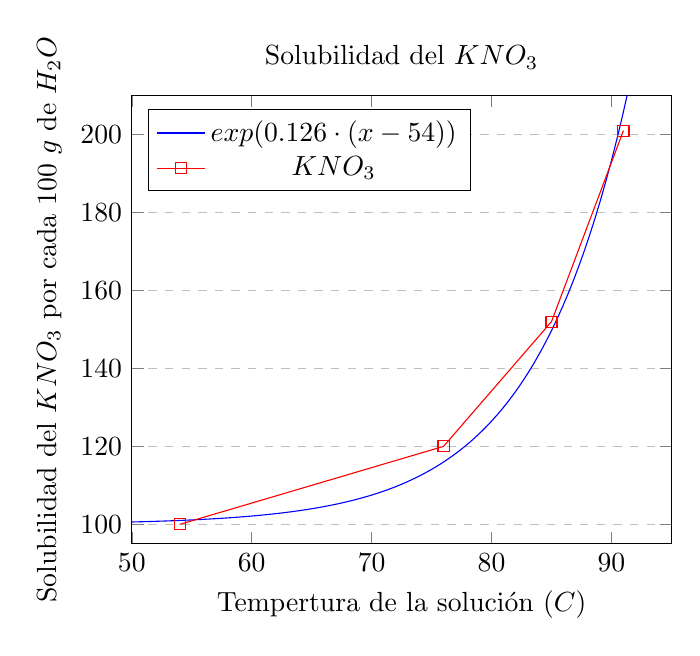
\begin{tikzpicture}
        \begin{axis}[
            title={Solubilidad del $KNO_3$},
            xlabel={Tempertura de la solución ($\degree C$)},
            ylabel={Solubilidad del $KNO_3$ por cada 100 $g$ de $H_2O$},
            xmin=50, xmax=95,
            ymin=95, ymax=210,
            xtick={50,60,70,80,90,100},
            %ytick={100,110,120,130,140,150,160,170,180,190,200},
            ytick={100,120,140,160,180,200},
            legend pos=north west,
            ymajorgrids=true,
            grid style=dashed,
        ]
            %exponential function
            \addplot[
                domain=50:95,
                color=blue,
                samples=100
            %]{-8.7981*10^(-10)*(x^6) + 6.2684*10^(-7)*(x^5) - 0.0000866718*(x^4) + 0.00362603*(x^3)};
            ]{exp(0.126*(x-54)) + 100};
            %\addlegendentry{\(-8.8\cdot10^{-10}x^6 + 6.3\cdot10^{-7}x^5 - 8.7\cdot10^{-5}x^4 + 3.6\cdot10^{-3}x^3\)}
            \addlegendentry{$exp(0.126\cdot(x-54))$}
            %data from table
            \addplot[
                color=red,
                mark=square,
            ]
            coordinates{ (54,100)(76,120)(85,152)(91,201)};
            \addlegendentry{$KNO_3$}
        \end{axis}
    \end{tikzpicture}
\end{center}

\subsection{Experimento 2}

\textit{Reacción del $H_2O$ con el $HCl$:}
\[H_2O_{(l)} \: + HCl_{(ac)} \rightarrow \: H_3O^+_{(ac)} \: + Cl^-_{(ac)} \]
Para hallar el volumen necesario de $HCl$ 2 M para diluirlo a 1 M
usaremos la siguiente ecuación:
\[
    V_1\cdot M_1 = V_2\cdot M_2
\]
Reemplazando:
\[V_{\acute{a}cido\:concentrado}\cdot 2\,M = 100\,mL\cdot1\,M\]
\[V_{\acute{a}cido\:concentrado}\,=\,50\,mL \]

Deduciendo sabemos que tenemos que añadir 50 $mL$ de agua
destilada al $HCl$ 2 M para así obtener $HCl$ 1 M. 

\subsection{Experimento 3}

\textit{Reacción del $H_2O$ con el $NaOH$:}
\[
    H_2O_{(l)} + NaOH_{(s)} \rightarrow Na^+_{(ac)} + OH^-_{(ac)} + H_2O_{(l)}
\]
Para hallar la cantidad necesaria de $NaOH$, usaremos las siguientes ecuaciones:
\begin{equation} \label{molaridad_eq}
    \eta_{NaOH} = V_{NaOH}\cdot M_{NaOH}
\end{equation}
\begin{equation} \label{molar_mass_eq}
    m_{NaOH} = \eta_{NaOH}\cdot \overline{M}_{NaOH}
\end{equation}
Reemplazando \ref{molaridad_eq} en \ref{molar_mass_eq}:
\begin{equation} \label{resultant_eq}
    m_{NaOH} = V_{NaOH}\cdot M_{NaOH}\cdot \overline{M}_{NaOH}
\end{equation}
Reemplazando con los valores numéricos:
\[
    m_{NaOH} = 100\cdot10^{-3}\,L\cdot0.1\,\frac{mol}{L}\cdot 40\frac{g}{mol}
\]
\[  m_{NaOH} = 0.4\,g\]
Entonces usando esa cantidad de $NaOH_{(s)}$ obtenemos la solución con la molaridad deseada.

La concentración de la solución de determinó de la siguiente manera:

\[ [NaOH] = 0.40\,g\cdot \frac{1\,mol}{40\,g}\cdot\frac{1}{0.1\,L}\]
\[ [NaOH] = 0.1\,M\]

\end{document}